%% -*- coding:utf-8 -*-
\begin{figure}
\centering

\ifpdf
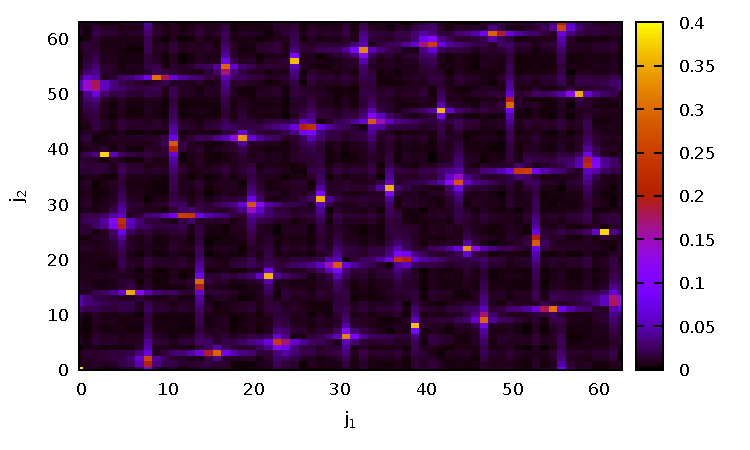
\includegraphics[angle=0]
{./part4/quantcomp/picellipticdiscretlog2.pdf}
\else
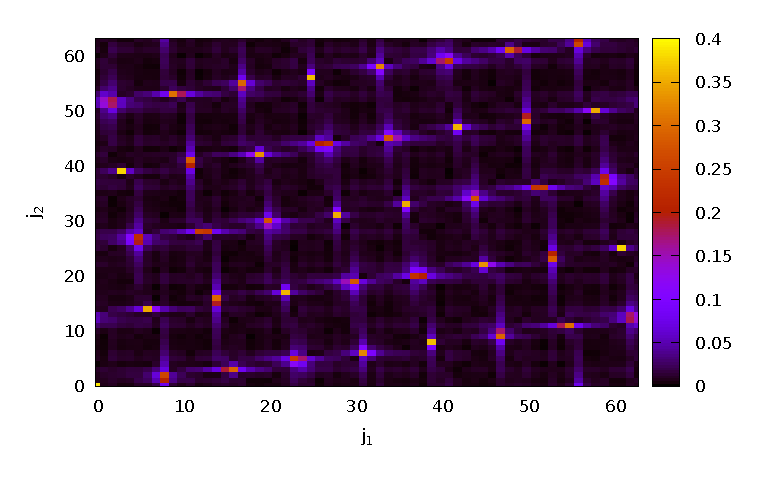
\includegraphics[angle=0]
{./part4/quantcomp/picellipticdiscretlog2.eps}
\fi

%\input ./part4/quantcomp/picdiscretlog2.tex

\caption{Fourier transform of the samples of the function 
$f'(x_1, x_2)$.
Number of samples $M=64$. The three bottom left maxima have coordinates approximately $(8,2), (15,3), (24,5)$, which gives the following estimates for $x$: $x \approx 4, 5, 4.8$,
which is close to the true value $x = 5$
} 
\label{fig:part4:quantcomp:dle2}
\end{figure}